% Copyright 2026 Sreeram Anil
% SPDX-License-Identifier: CC-BY-4.0
% =============================================================================
%  Decentralised pack filtering with the reduced-order cell model — pack family
% =============================================================================
\chapter{Decentralised Reduced-Order Pack Filter (Decentralized-ReducedEKF)}
\label{ch:decentralizedreducedekf}

\section*{At a glance}
\begin{tabular}{@{}l>{\raggedright\arraybackslash}p{0.76\textwidth}@{}}
Family & pack-level (baseline variant: no information exchange) \\
Header & \texttt{include/estkit/pack/pack\_common.hpp} (\texttt{DecentralizedPackM}) \\
 & + \texttt{battery/ecm\_model\_reduced.hpp} \\
Registered name & \texttt{Decentralized-ReducedEKF} \\
Structure & $N_c$ independent 3-state EKFs, $\vx=[\soc,v_1,h]^\T$ \\
Cost per step & \SI{2775}{\nano\second} for $N_c=12$ cells (\SI{231}{\nano\second} per cell) \\
Memory & \SI{51264}{\byte} $= N_c\times\SI{4272}{\byte}$ \\
Bus load & 0 \\
Primary references & \cite{simon2006,plett2016bms2,plett2004ekf3} \\
\end{tabular}

\section{Motivation and aerospace/BMS relevance}
If a pack BMS cannot afford $N_c$ four-state filters, the cheapest lever short of changing the
architecture is to shorten the state vector. The reduced-order ESC model
(\texttt{EcmModelReduced}, Chapter~\ref{ch:reducedorderekf}) removes the slow RC branch from the
state and reconstructs it quasi-statically from the current history, leaving
$\vx=[\soc,v_1,h]^\T$. Every covariance operation then costs $(3/4)^3=\num{0.42}$ of the full
model's, and the missing dynamics are accounted for by an additional measurement-noise term
following Simon's treatment of reduced-order Kalman filtering \cite[Ch.~10]{simon2006}.

This chapter registers that model in the decentralised pack architecture, and it is included for
two reasons. First, it is the cheapest per-cell estimator in the family and therefore the right
comparison point for \estname{BarDelta}, which is cheaper still. Second, it demonstrates a general
lesson for pack design: \emph{reducing the model} and \emph{reducing the architecture} are not
interchangeable. Dropping one state saves \SI{29}{\percent} of the arithmetic and costs
\SI{47}{\percent} of the accuracy; changing the architecture from decentralised to common-state
saves \SI{86}{\percent} of the arithmetic and \emph{gains} \SI{52}{\percent} of the accuracy.

\section{Problem statement and assumptions}
As in Chapter~\ref{ch:decentralizedekf}, but each cell filter carries
\begin{equation}
\vx_{j,k} = [\soc_{j,k},\,v_{1,j,k},\,h_{j,k}]^\T\in\real^{3},
\label{eq:dre-state}
\end{equation}
and the slow branch is an internal, non-estimated signal of the model,
\begin{equation}
v_{2,j,k+1}^{\text{qs}} = a_2 v_{2,j,k}^{\text{qs}} + R_2(T)(1-a_2)\,i_k,\qquad a_2=e^{-\dt/\tau_2(T)},
\label{eq:dre-v2qs}
\end{equation}
driven open loop by the measured current.

\begin{assumption}[Uncorrectable slow branch]\label{as:dre-slow}
$\tau_2\approx\SI{120}{\second}$ is long compared with the correlation time of the SOC
information in a single terminal-voltage channel, so $v_2$ is nearly unobservable from $v$ alone;
removing it from the state costs little \emph{provided} $R_2$ and $\tau_2$ are accurate.
\end{assumption}
\begin{assumption}[Reconstruction error as noise]\label{as:dre-noise}
The residual $v_{2}^{\text{true}}-v_2^{\text{qs}}$ is modelled as an extra white measurement noise
\cite[Ch.~10]{simon2006},
\begin{equation}
R = \sigma_v^2 + (R_0\sigma_i)^2 + \sigma_{v_2}^2 ,
\label{eq:dre-R}
\end{equation}
with $\sigma_{v_2}=\SI{2}{\milli\volt}$ the library default. It is in truth strongly
\emph{coloured} --- it is a first-order lag of the parameter error times the current --- and this
is where the accuracy is lost.
\end{assumption}

\section{Derivation}
The filter is the EKF of Chapter~\ref{ch:ekf} applied to \texttt{EcmModelReduced}, whose analytic
Jacobians are
\begin{equation}
\mF = \diag\big(1,\;a_1(T),\;a_h(i)\big),\qquad
\mH = \big[\;\ocv'(\soc,T)\;\;-1\;\;M\;\big],
\label{eq:dre-jac}
\end{equation}
and whose output equation carries the reconstructed branch,
$h(\vx,\vu)=\ocv(\soc,T)+Mh-v_1-v_2^{\text{qs}}-R_0(T)i$. Equation \eqref{eq:dre-v2qs} is advanced
inside $f$, so the model requires a filter that evaluates $f$ exactly once per sampling period ---
the EKF family. A sigma-point or particle filter, which evaluates $f$ once per sample point, would
advance \eqref{eq:dre-v2qs} $2n_x+1$ times per step and corrupt it. This constraint is documented
in the model header and is the reason no \texttt{Decentralized-ReducedUKF} exists.

\paragraph{Why it needs a new pack wrapper.} \texttt{DecentralizedPack<Filter>} of
\texttt{pack\_estimator.hpp} instantiates \texttt{CellEstimator<Filter>}, whose model parameter
defaults to \texttt{EcmModel}; with \texttt{Filter = Ekf<EcmModelReduced>} the adapter would try to
build a 3-state filter from a 4-state model and would not compile. \texttt{DecentralizedPackM<Filter,Model>}
in \texttt{pack\_common.hpp} is the same container with the model type made
explicit, and is the wrapper used here.

\section{Algorithm}
Identical to Chapter~\ref{ch:decentralizedekf} with $n_x=3$, the Jacobians \eqref{eq:dre-jac},
the noise \eqref{eq:dre-R}, and the extra internal recursion \eqref{eq:dre-v2qs} executed once per
time update.

\section{Application to the battery model}
\texttt{DecentralizedPackM<Ekf<EcmModelReduced>, EcmModelReduced>} with the model's own defaults:
$\sigma_{v_2}=\SI{2}{\milli\volt}$, $\mP_0 = \diag(\sigma_{\soc_0}^2, (\SI{2}{\milli\volt})^2,
\num{0.25})$, process-noise floors $(\num{1e-5},\num{1e-4},\num{1e-3})$. The pack dataset gives the
estimator the nominal parameter set, so $R_2$ and $\tau_2$ in \eqref{eq:dre-v2qs} are the module
averages while each cell's true $R_2$ deviates by the manufacturing spread
($\sigma=\SI{8}{\percent}$, and $R_2$ is \emph{not} scaled with $R_0$ in the aged cell), which is
exactly the mismatch Assumption~\ref{as:dre-noise} has to absorb.

\section{Implementation notes}
$N_c$ \texttt{Ekf<EcmModelReduced>} objects of \SI{4272}{\byte} each. The saving over the full
model is only \SI{64}{\byte} per cell in this library because the OCV table
(\SI{3872}{\byte}) dominates \texttt{sizeof}; the \emph{covariance} storage falls from
$4^2$ to $3^2$ reals and the arithmetic from \SI{322}{\nano\second} to \SI{231}{\nano\second} per
cell, a \SI{29}{\percent} saving that matches the $(3/4)^3$ estimate for the cubic terms diluted
by the model evaluations. \texttt{v2\_} is a \texttt{mutable} member of the model and is copied
with it, so each cell owns its own reconstruction --- correct, since the cells have different
temperatures.

\section{Benchmark results}
% Copyright 2026 Sreeram Anil
% SPDX-License-Identifier: CC-BY-4.0
\begin{table}[H]\centering\footnotesize\setlength{\tabcolsep}{4pt}\caption{Decentralized-ReducedEKF: pack-level benchmark (12-cell module, eVTOL mission, mean over seeds; all errors in \% SOC). RMSE$_\mathrm{cells}$: per-cell RMSE over all cells; RMSE$_{\min/\mathrm{mean}/\max}$: error of the weakest / mean / strongest-cell SOC; 51264 bytes of state, 0 numbers exchanged per step.}\label{tab:pack_DecentralizedReducedEKF}
\begin{tabular}{lrrrrrrcr}\toprule scenario & RMSE$_\mathrm{cells}$ & RMSE$_{\min}$ & RMSE$_\mathrm{mean}$ & RMSE$_{\max}$ & max cell err. & RMSE$_\mathrm{ss}$ & div. & ns/step \\ \midrule
nominal & 1.81 & 1.86 & 0.57 & 1.48 & 11.59 & 1.41 & no & 4190 \\
init\_error & 1.81 & 1.86 & 0.57 & 1.48 & 11.59 & 1.41 & no & 4094 \\
current\_bias & 1.89 & 1.68 & 0.79 & 2.01 & 9.62 & 1.48 & no & 4152 \\
weak\_cell & 2.46 & 5.53 & 0.92 & 1.49 & 21.01 & 1.86 & no & 4134 \\
noise\_step & 1.81 & 1.86 & 0.57 & 1.49 & 11.59 & 1.41 & no & 4136 \\
large\_imbalance & 1.83 & 1.33 & 0.61 & 0.96 & 11.55 & 1.40 & no & 4101 \\
\bottomrule\end{tabular}\end{table}

\begin{figure}[H]\centering
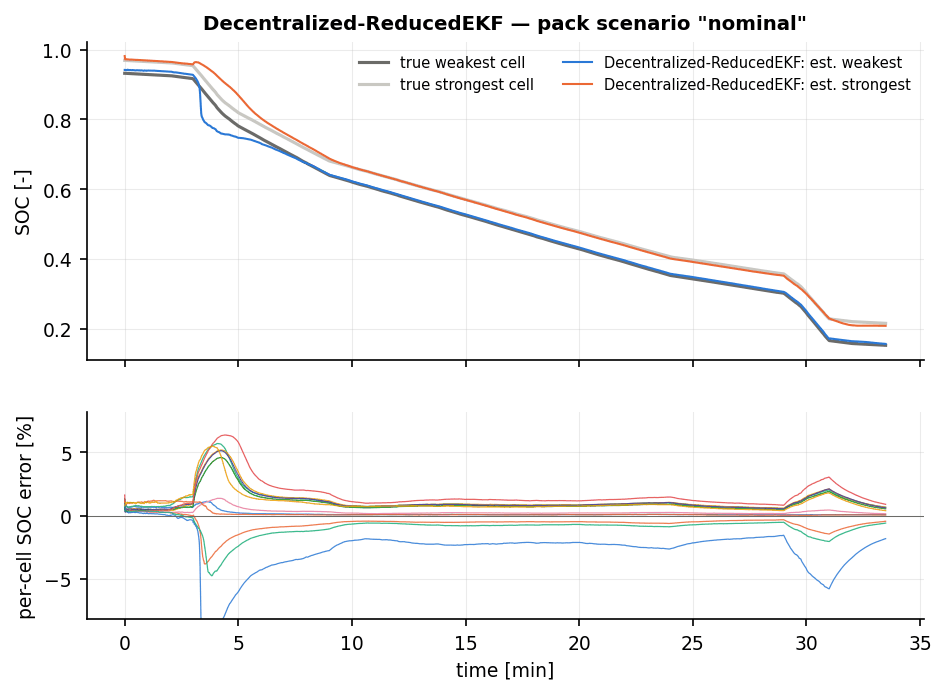
\includegraphics[width=\textwidth]{figures/pack_DecentralizedReducedEKF_nominal.png}
\caption{Decentralized-ReducedEKF on the nominal eVTOL mission: the open-loop slow branch
\eqref{eq:dre-v2qs} produces a current-correlated error visible during the high-power segments.}
\end{figure}
\begin{figure}[H]\centering
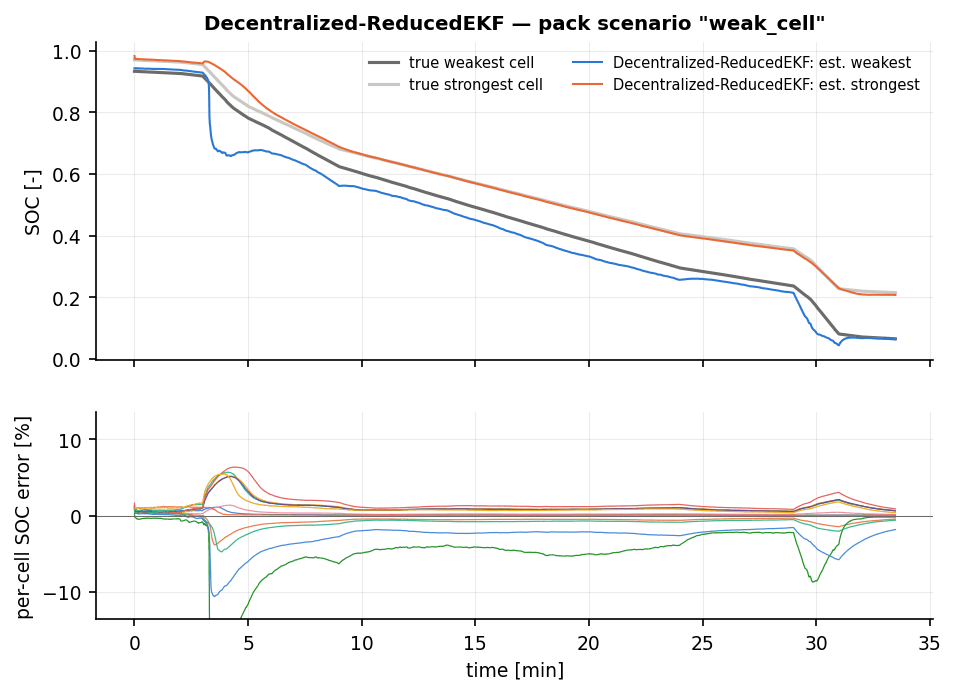
\includegraphics[width=\textwidth]{figures/pack_DecentralizedReducedEKF_weak_cell.png}
\caption{Decentralized-ReducedEKF on \texttt{weak\_cell}: the aged cell's $R_2$ is not scaled with
its other resistances, so the quasi-static reconstruction is worst exactly there.}
\end{figure}

Means over three seeds, against the full-order version of the same architecture:
\begin{center}\small
\begin{tabular}{@{}lcccc|cccc@{}}
\toprule
& \multicolumn{4}{c|}{\estname{Decentralized-ReducedEKF}} & \multicolumn{4}{c}{\estname{Decentralized-EKF}} \\
Scenario & rmse & rmse$_{\min}$ & ss & max & rmse & rmse$_{\min}$ & ss & max \\
\midrule
\texttt{nominal}          & 0.0181 & 0.0186 & 0.0141 & 0.116 & 0.0123 & 0.0081 & 0.0134 & 0.046 \\
\texttt{init\_error}      & 0.0181 & 0.0186 & 0.0141 & 0.116 & 0.0118 & 0.0082 & 0.0129 & 0.042 \\
\texttt{current\_bias}    & 0.0189 & 0.0168 & 0.0148 & 0.096 & 0.0137 & 0.0088 & 0.0148 & 0.056 \\
\texttt{weak\_cell}       & 0.0246 & 0.0553 & 0.0186 & 0.210 & 0.0129 & 0.0129 & 0.0137 & 0.048 \\
\texttt{noise\_step}      & 0.0181 & 0.0186 & 0.0141 & 0.116 & 0.0122 & 0.0084 & 0.0131 & 0.045 \\
\texttt{large\_imbalance} & 0.0183 & 0.0133 & 0.0140 & 0.116 & 0.0174 & 0.0245 & 0.0179 & 0.061 \\
\midrule
\si{\nano\second}/step & \multicolumn{4}{c|}{2775} & \multicolumn{4}{c}{3860} \\
bytes & \multicolumn{4}{c|}{51264} & \multicolumn{4}{c}{52032} \\
\bottomrule
\end{tabular}
\end{center}

\paragraph{It meets the acceptance criteria but is the weakest estimator of the family.} The
steady-state error \num{0.0141} is below the \num{0.02} threshold in every scenario and nothing
diverges in eighteen runs, but the total \texttt{rmse} (\num{0.0181}) and especially the worst
single-cell error (\num{0.116}) are the largest here. The error is not random: the open-loop
branch \eqref{eq:dre-v2qs} is driven by the \emph{measured} current with the \emph{nominal}
$R_2,\tau_2$, so during the \num{4.5}C hover segments the reconstruction is wrong by
$\Delta R_2 i\approx\SI{18}{\milli\volt}$ for a cell whose $R_2$ deviates by \SI{8}{\percent},
nine times the sensor noise, and the filter converts that into SOC. The \texttt{max} column
records the peaks of those transients.

\paragraph{Insensitivity to the scenario is diagnostic, not a virtue.} \texttt{nominal},
\texttt{init\_error} and \texttt{noise\_step} give \emph{identical} figures to four digits. The
three scenarios share the same current and voltage records up to the initial SOC guess
(\texttt{init\_error}) and the sensor-noise level after \SI{600}{\second}
(\texttt{noise\_step}); the fact that neither perturbation is visible means the error is entirely
dominated by the deterministic model-reduction residual and not at all by the sensor noise or the
initial condition. That is the signature of a systematic, not a stochastic, error, and it is
exactly what Assumption~\ref{as:dre-noise} gets wrong: a coloured residual modelled as white
noise.

\paragraph{\texttt{weak\_cell} is its worst case.} The benchmark's aged cell has $R_0$ and $R_1$
scaled by \num{1.3} but $R_2$ unchanged, so the nominal $R_2$ used by \eqref{eq:dre-v2qs} is
relatively \emph{more} wrong for that cell than for the others; \texttt{rmse}$_{\min}$ rises to
\num{0.0553} and the worst single-cell error to \num{0.210}. A pack BMS that reduces the cell
model must therefore identify $R_2$ per cell --- which is precisely what the delta-impedance state
of Chapter~\ref{ch:bardelta} does, at a fraction of the cost of a per-cell state.

\paragraph{Reduce the architecture, not the model.} Side by side on \texttt{nominal}:
\begin{center}\small
\begin{tabular}{@{}lccc@{}}
\toprule
& rmse & \si{\nano\second}/step & bytes \\
\midrule
\estname{Decentralized-EKF} (4-state, $N_c$ filters)        & 0.0123 & 3860 & 52032 \\
\estname{Decentralized-ReducedEKF} (3-state, $N_c$ filters) & 0.0181 & 2775 & 51264 \\
\estname{BarDelta} (1 full filter + $N_c$ 3-state deltas)   & 0.0059 &  542 &  5616 \\
\bottomrule
\end{tabular}
\end{center}
Model reduction saves \SI{29}{\percent} of the time and costs \SI{47}{\percent} of the accuracy;
the common-state architecture saves \SI{86}{\percent} of the time and gains \SI{52}{\percent} of
the accuracy. For a series pack the architecture is by far the more effective lever, and this row
is the quantitative justification for the rest of the family.

\section{Summary}
Use the reduced-order cell model in a pack only when the slow-branch parameters are trustworthy
per cell and memory per filter --- not accuracy --- is the binding constraint; it delivers the
cheapest per-cell EKF in this library and never diverges, but its error is dominated by a coloured
model-reduction residual that the white-noise inflation \eqref{eq:dre-R} cannot represent, and that
residual is worst exactly for the aged cell a BMS cares most about. Note also that the model
carries an internal recursion, so it is restricted to filters that evaluate $f$ once per sample.
If the goal is to cut the pack budget, cut the architecture instead: bar-delta filtering is seven
times cheaper \emph{and} three times more accurate than this variant.
